\documentclass{article}
\usepackage[framemethod=tikz]{mdframed}
\mdfdefinestyle{mystyle}{%
  rightline=true,
  innerleftmargin=10,
  innerrightmargin=10,
  outerlinewidth=3pt,
  topline=false,
  rightline=true,
  bottomline=false,
  skipabove=\topsep,
  skipbelow=\topsep
}
\title{Configuration and Verification of LSIT Setup \\
\large Used for confirming proper alignment and signal level of photodiodes used for measuring laser timing}
\author{Justin May}
\date{2023-10-12}
\begin{document}
\maketitle

\section{Introduction}
The Laser Interface Module (LSIT) is a SLAC built module that combines numerous functions. When we originally designed it, we referred to it as the garbage can module because it's where we put all the extra functionality that we needed. Early modules included an amplifier chain necessary for raising a carrier signal to the level needed for typical phase noise measurements. Later versions include pulse stretchers for making it easier for a laser operator to look at the very fast signals from detectors.

The primary function that the module carries out is precisely converting the analog signal from a photodiode looking at the output of a pulsed laser, for all intents a delta function when dealing with general lab equipment, to a fixed amplitude logic-like output. High speed rf components preserve the temporal characteristics of the pulse, with a very fast risetime, but keep the output level high long enough for lab equipment (in particular a precision time-interval counter) to capture on the signal. Finally, after sufficient duration, a reference trigger that the laser time is being measured against also resets the device, in preparation for the next laser pulse.

\section{Typical Setup}
Two typical setups used on lasers throughout the facility are shown below.
\begin{figure}[h]
    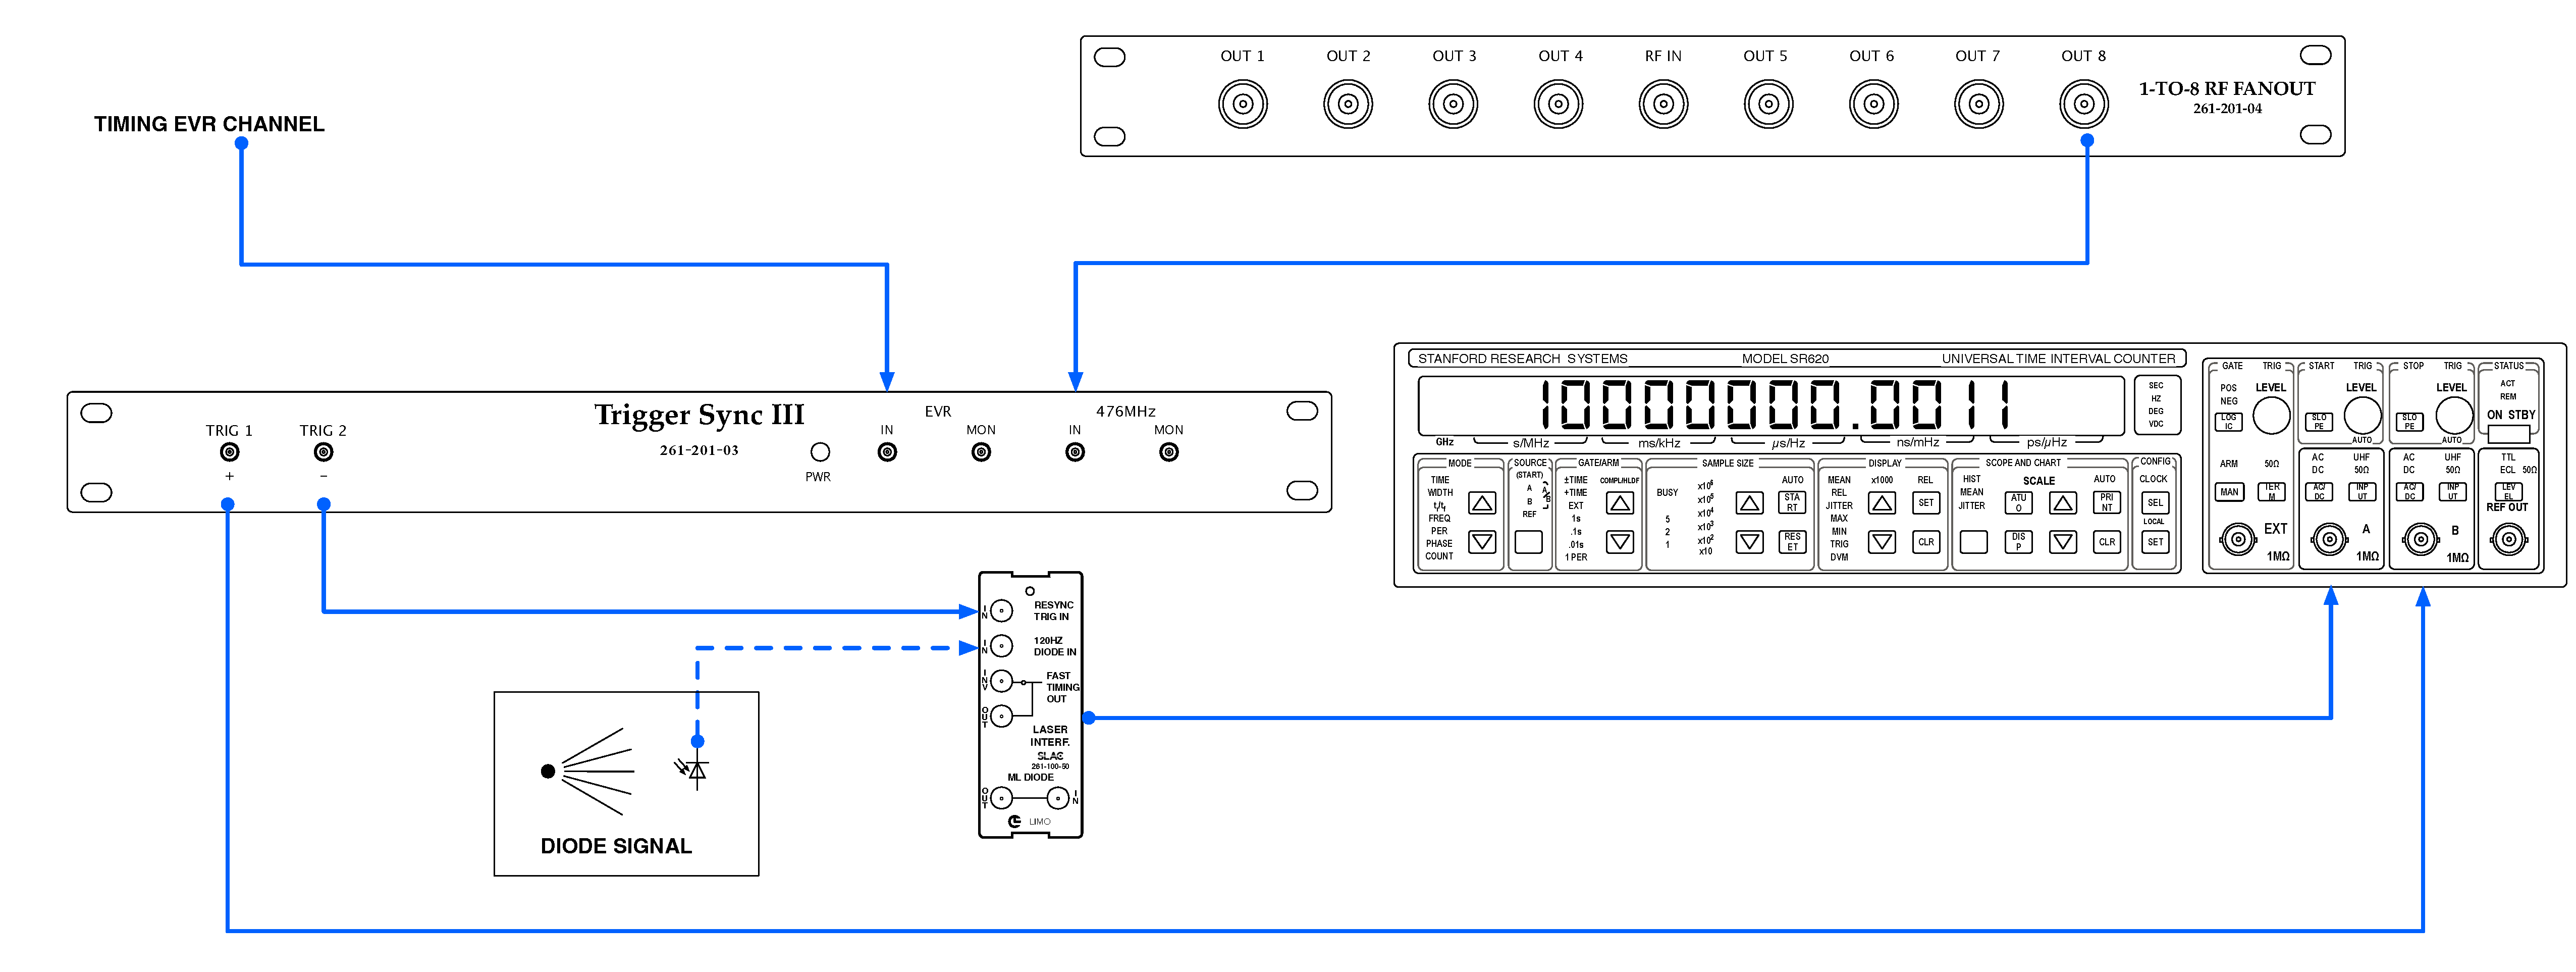
\includegraphics[width=\textwidth]{rsc/sampleconnections.pdf}
    \caption{LSIT used with a Coherent Vitara/Evo}
\end{figure}
\begin{figure}[h]
    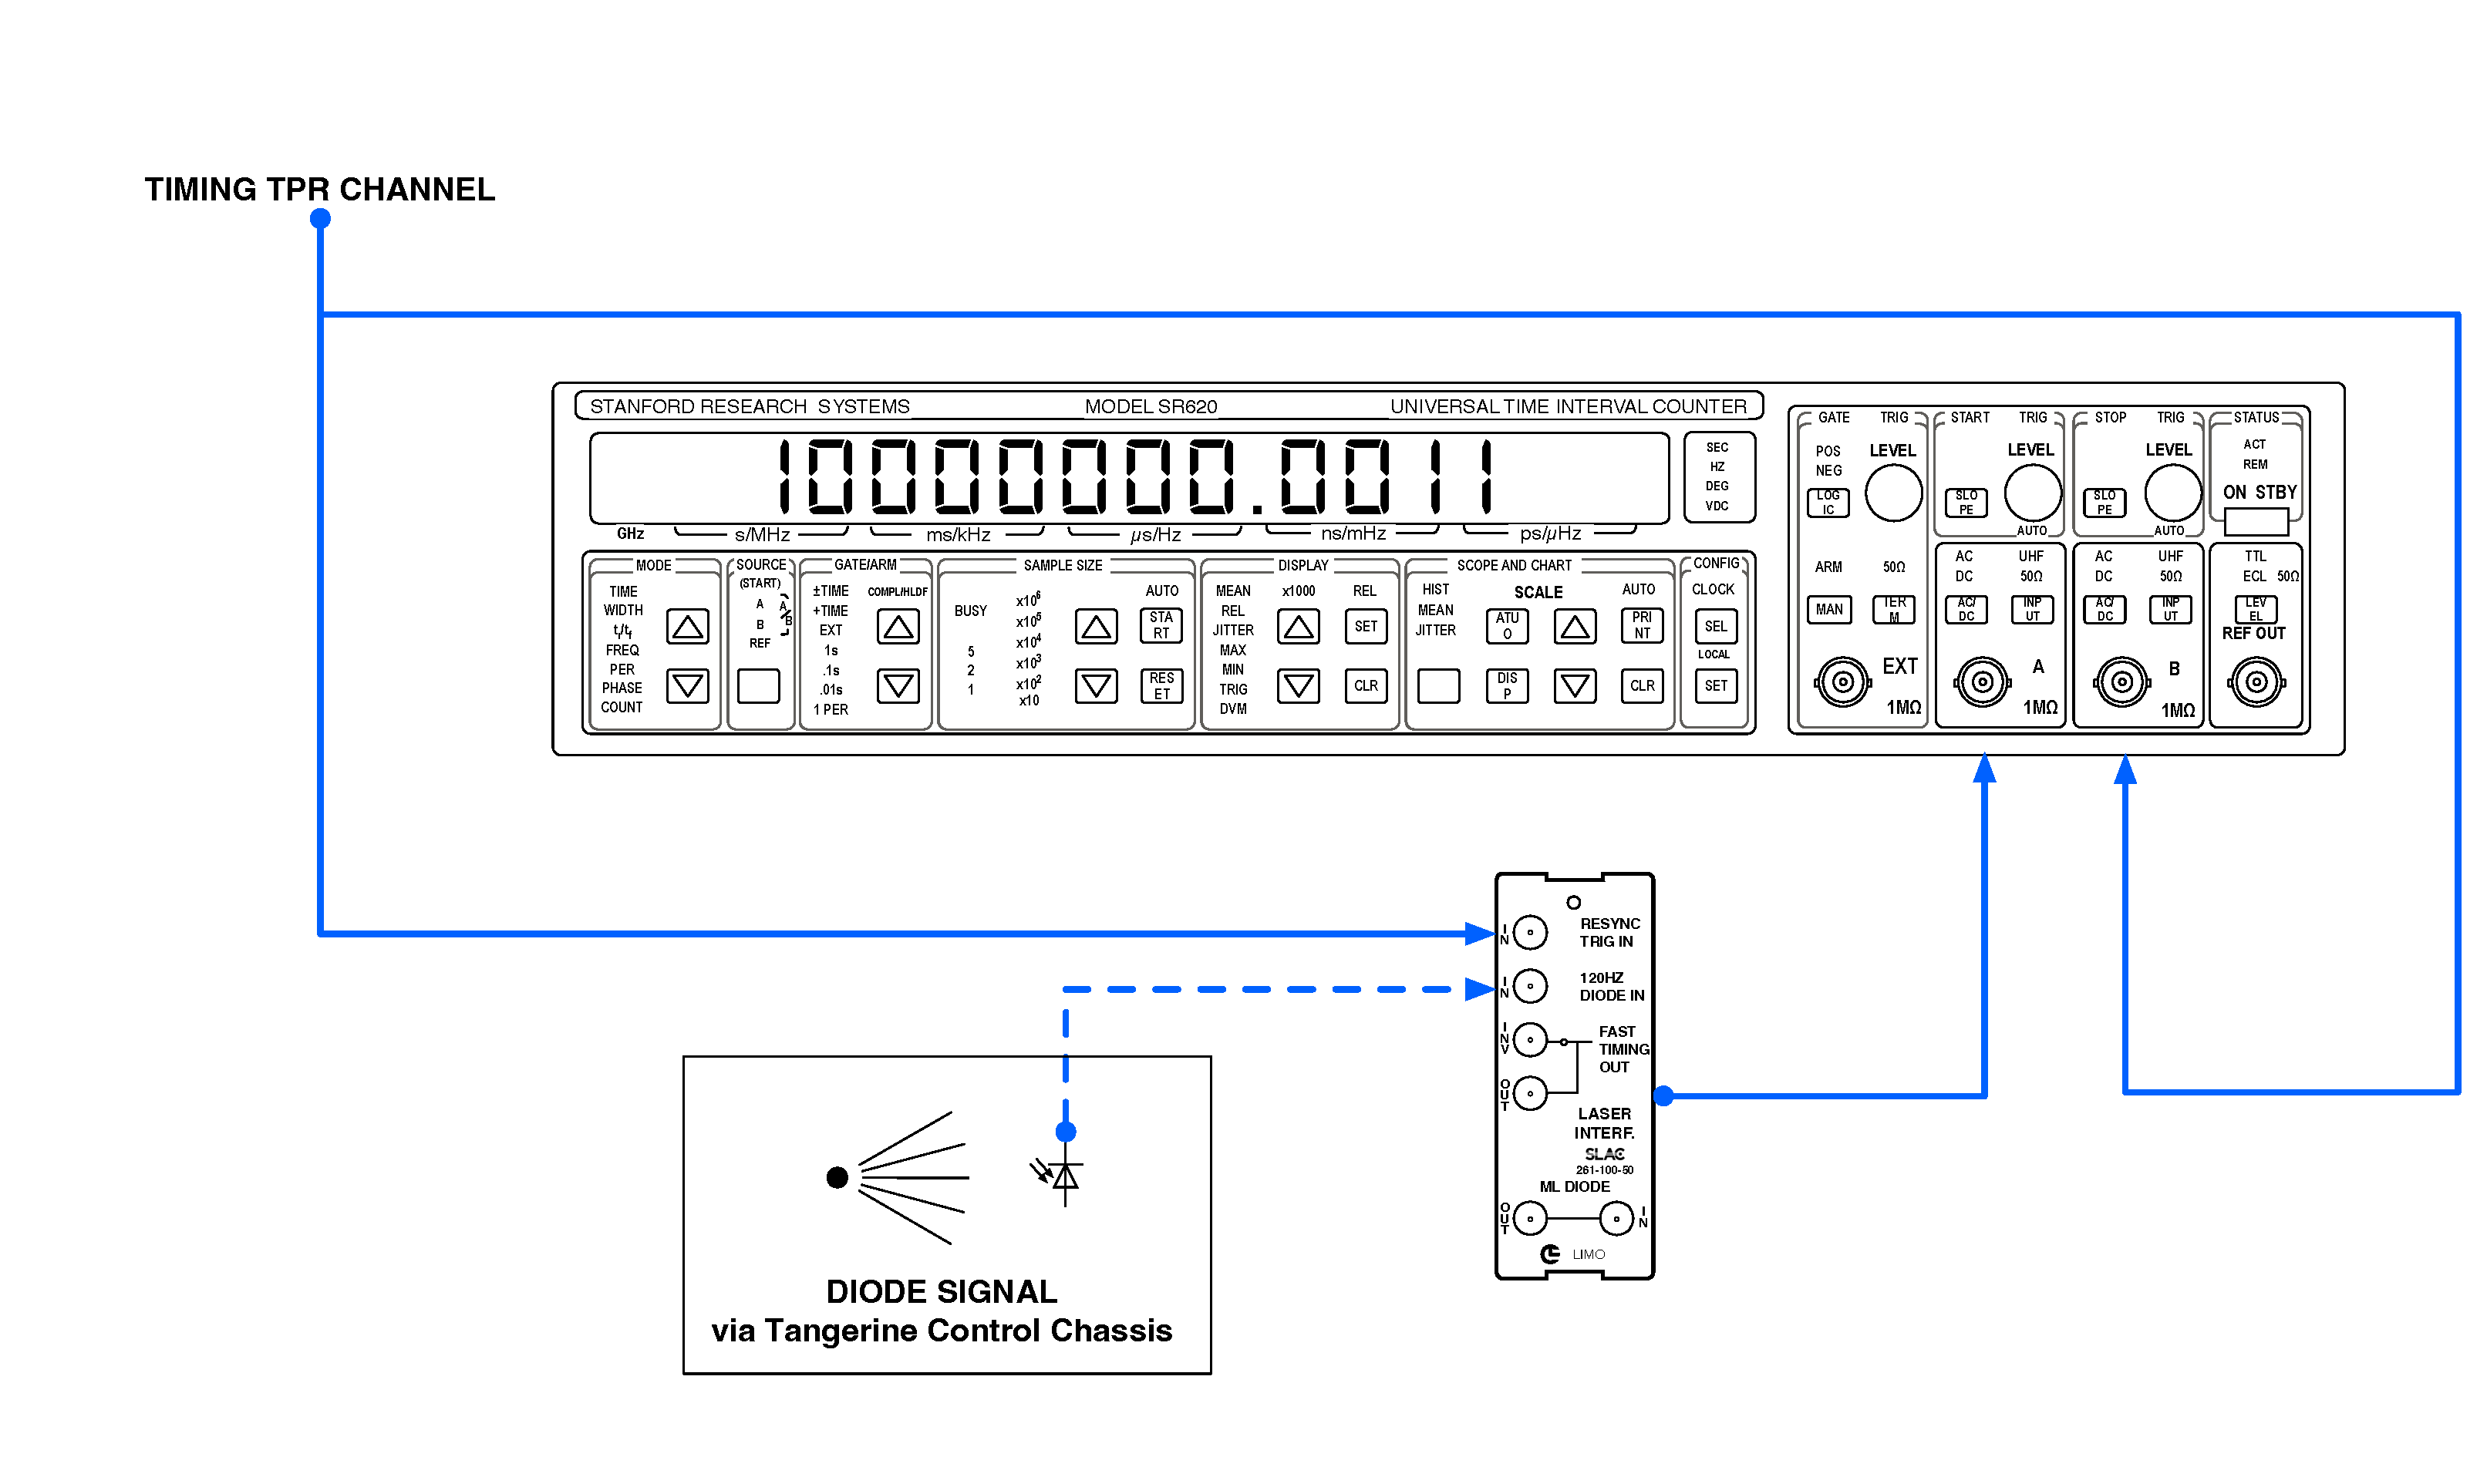
\includegraphics[width=\textwidth]{rsc/sampleconnections_tangerine.pdf}
    \caption{LSIT used with an Amplitude Tangerine}
\end{figure}
\begin{mdframed}[style=mystyle,frametitle=Note on Tangerines]
    The integrated photodiode in the Tangerine has a lower output level than the 'traditional' Vitara, and so input scaling needed to be modified for the units used on the Sector 0 lasers. Similarly, the Sector 0 lasers were commissioned without using Trigger Re-Sync modules, in part because the performance of the TPRs was good enough. However, the TPR output is a positive output, and so the polarity of the module also needed to be changed.
    \end{mdframed}

When initially connecting the LSIT module or troubleshooting a system, the module output can be checked without a reset trigger connected. In this case, one should observe a square wave with frequency of $\frac{1}{2}*F_{amplifier}$ (see figure \ref{noreset}).
\begin{figure}[h]
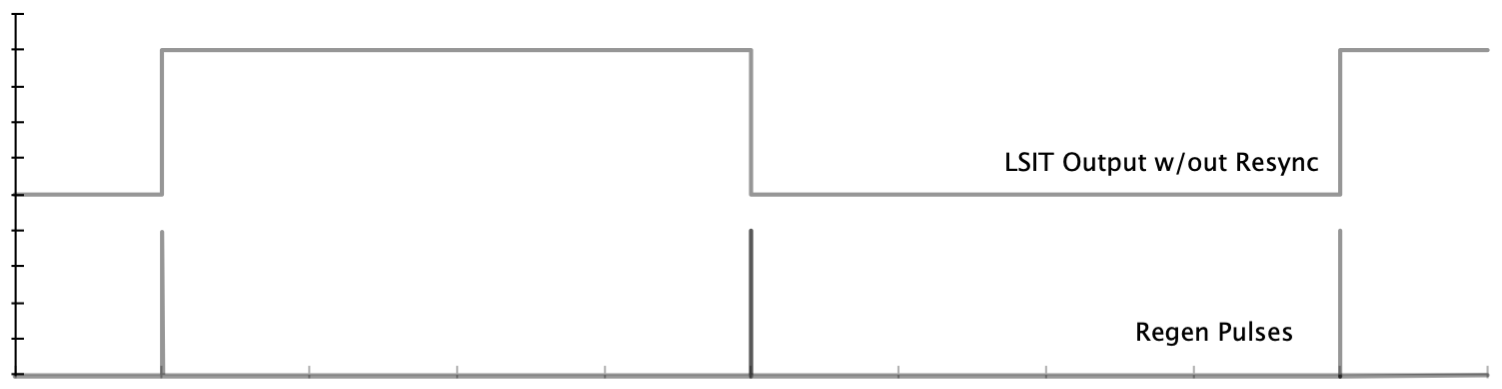
\includegraphics[width=\textwidth]{rsc/LSIT_withoutreset.png}
\caption{LSIT with proper amplifier signal and no reset trigger}\label{noreset}
\end{figure}

If the user then connects a reset trigger (typically a copy of the reference trigger the laser is measured against), then the output should change to a pulse with frequency equal to $F_{amplifier}$ and pulse width equal to the delta between the laser pulse and the reset trigger, minus some negligible propagation time (see figure \ref{reset}). 
\begin{figure}[h]
    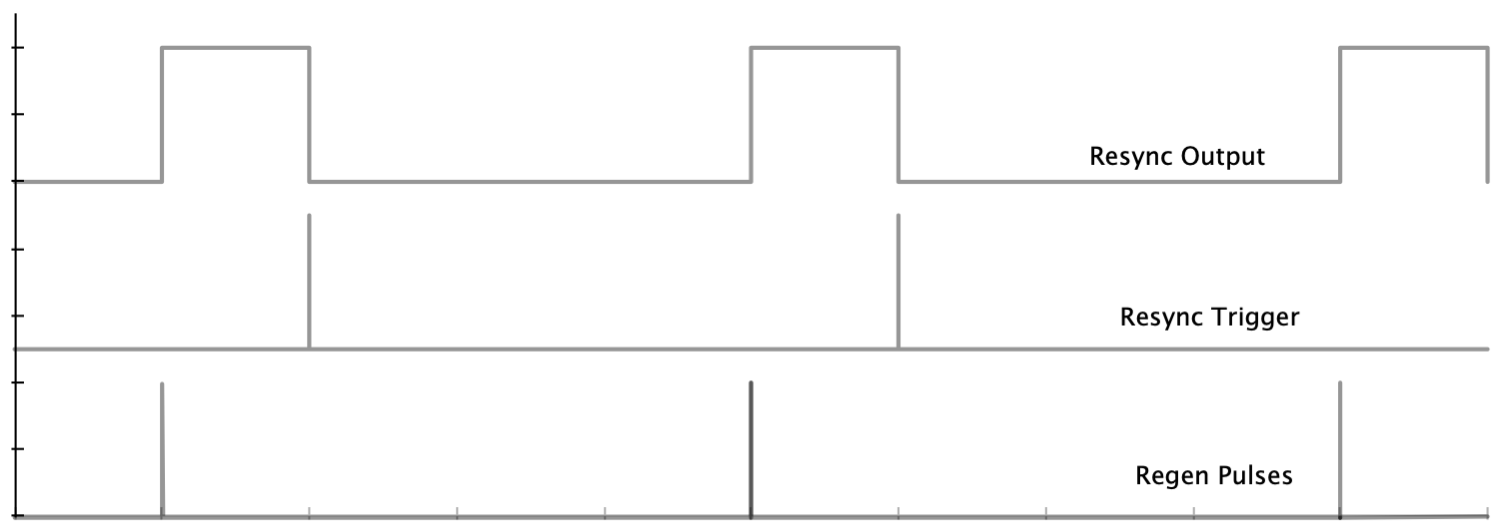
\includegraphics[width=\textwidth]{rsc/LSIT_withreset.png}
    \caption{LSIT with proper amplifier signal and reset trigger}\label{reset}
    \end{figure}

\section{Incorrect Signal Levels}
A laser that requires the use of an LSIT has a pulse width that is typically difficult to otherwise measure. If not, there'd be no need for the module in the first place. However, particularly if the photodiode being used to measure the output time of the amplifier is separate from the laser assembly, it can be difficult to align the photodiode and set the proper signal intensity. After rough alignment using traditional alignment techniques, it's natural to put the photodiode signal on an oscilloscope to optimize the pointing and signal level.

An extremely fast signal into a reactive load is modulated by the effective response function of the load. In other words, when the photodiode signal is connected to a scope that is available to the laser operator, the observed output will vary depending on the channel bandwidth. The slower the scope, the lower and slower the diode signal will appear to be.

The design of the LSIT is, unfortunately, sensitive to having the correct level, and so setting the signal level really should be done with the output of the LSIT on a scope. With this setup, the correct output will be a clean square pulse as shown in figure \ref{reset}. However, when the signal level is too high or too low, the LSIT output will result in invalid timing measurements. In the worst case, an invalid timing measurement can be detected as a bucket jump, and the laser timing controls will attempt to correct the jump, erroneously moving the laser away from the intended operating point.

\begin{figure}[h]
    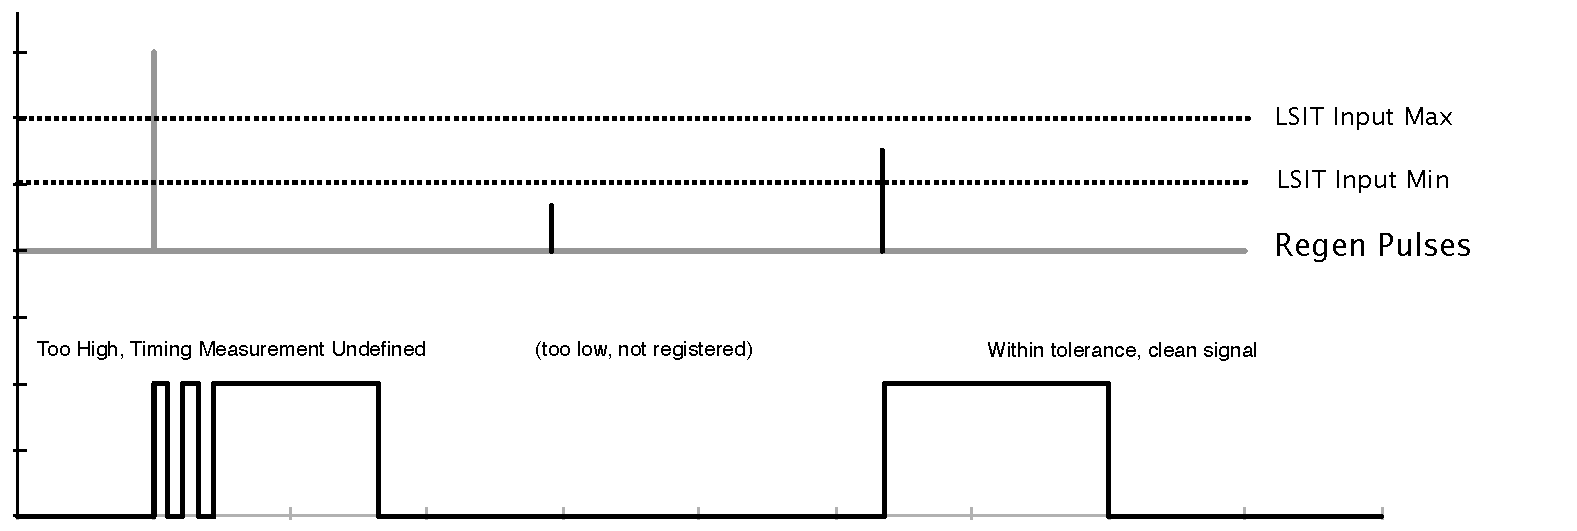
\includegraphics[width=\textwidth]{rsc/LSIT_signalrange.pdf}
    \caption{LSIT response for various signal levels}\label{signallevels}
    \end{figure}
    
In figure \ref{signallevels}, the first pulse is represented as above the LSIT max threshold. In this case, the LSIT will retrigger on the large input pulse. To identify this, with the LSIT output on a scope (one can use the complementary output for this to keep from disconnecting from a time interval counter), reduce the timebase to the nanosecond scale and look at the leading edge of the pulse. If multiple edge transitions are visible, the signal level on the photodiode should be reduced.

If, however, the signal level is too low, as shown in the second pulse in figure \ref{signallevels}, the LSIT will never trigger.

It is important to note that, in the first case where the signal level is too high, there is no guarantee at which level the LSIT will end up after the burst of edge transitions. If the operator has the oscilloscope zoomed out and there were an even number of edge transitions, the LSIT will settle at the no output level, and the transitions are fast enough that they will be aliased out of the scope image (unless, for instance, a Peak Detection mode is enabled). The take away is that when checking signal levels on a scope, get in the habit of adjusting the timebase back and forth between ns and us scales.

\section{Oscilloscope Response}
As mentioned above, the photodiode output from a short laser pulse depends on the response of the load attached to it. The output will look somewhat like the step response of a low pass filter with finite response. Figure \ref{scopecurves} shows response curves for various input pulses as a function of scope channel characteristics for the optimal LSIT input level. Table \ref{typicalranges} shows the input range for the LSIT for various representative scopes.
\end{document}